\chapter{Methods}
\label{chapter:methods}
This chapter describes our proposed solution. It is dived into the following blocks.

\medskip 
Section \ref{sec:caries_detection} describes the baseline solution. Particularly, we describe the training protocol used in remaining sections of the chapter.

\medskip Section \ref{sec:methods:improvements} introduces a few changes to the training protocol previously described in Section \ref{sec:caries_detection}.

\medskip Section \ref{sec:model_inspection} inspects how the behavior of trained models changes, if we choose a differently sized backbone or use different weight decay.

\medskip Section \ref{sec:model_ensemling} improves detection results by ensembling multiple models. Furthermore, we assess the importance of models used in the ensembling.

\medskip Section \ref{sec:methods:dental_restorations} proposes a deep learning and a non-deep learning approach to segmentation of dental restorations.

\section{Caries detection - baseline model comparison}
\label{sec:caries_detection}

Firstly, we implemented and tested multiple object-detection architectures and compared them against each other on the stage of the currently available dataset. The training protocol used throughout the training of all models is described by the following:

\subsection{Dataset}
We used the first five stages of the dataset mentioned in chapter \ref{chapter:dataset}. The dataset was split into training, validation, and test parts, consisting of 70\%, 15\%, and 15\% of the dataset.

\subsection{Image augmentations}
\label{sec:image_augmentations}
The image was augmented by a single pipeline that applied the following transformations with corresponding probabilities $p$.
\begin{itemize}
    \item Normalize the image by substracting the mean of the dataset and divide by standard deviation of the dataset (mean$=0.37$, std$=0.28$), $p=1$.
    \item Resize and pad to $1024\times1024/896$, $p=1$.
    \item Horizontal flip, $p=0.5$.
    \item Vertical flip, $p=0.5$.
    \item Rotation, $p=0.3$, rotation limit$=10^{\circ}$.
    \item Translation, $p=0.5$, translation limit$=10\%$ of the image size.
    \item Gaussian blur flip, $p=0.3$, kernel size from 7 to 31.
    \item Gamma correction, $p=0.3$, $\gamma$ in range from 0.6 to 1.4.
\end{itemize}
The results of those augmentations can be seen in appendix \ref{appendix:img_transformations}.

We selected the dimensions to which the image will be resized due to the limitations of some architectures, which require the input to be divisible by 128. In the beginning, we used square images due to the ease of implementation. After that, we switched to rectangular images, however no improvement in measured metrics was observed. Based on the architecture, we noticed a decrease in GPU memory usage in the range from 5\% to 10\%.k

\subsubsection{Computing power}
All the computations were realized on the CMP cluster, consisting of multiple GPU nodes, and the experiments were conducted on the Boruvka and Zorn machines. Both of them have 32 CPU cores, 256GB of RAM memory, and 8 NVIDIA GeForce GTX 1080-Ti graphics cards with 12GB of dedicated memory.

\subsection{Neural network models}
\label{sec:methods:nns}
Multiple architectures of neural networks were used. As the work on the thesis progressed, the amount grew larger; thus, a wider variety of models can be seen in the advanced stages of the dataset. We stopped using the YOLOv3 model after stage 2, since the YOLOv5 model had a superior performance on stages one and two, see tables \ref{tab:model_results:stage_one} and \ref{tab:model_results:stage_two}.

All the models we used and their respective backbones are listed below.
\begin{itemize}
    \item YOLOv3 with Darknet-53 backbone
    \item YOLOv5 with backbones with the sixth generation of backbones. We used the small, medium, large and extra large versions of those backbones. In further text, we will denote them as s6, m6, l6, and x6.
    \item Faster-RCNN with Resnet50 and Resnet101 backbone; R50 and R101 abbreviations will be used.
    \item RetinaNet (RetN) with Resnet50 and a tiny swin transformer (swint) backbones.
    \item EfficientDet with D0,D1,D2,D3,D4 and D5 backbones.
\end{itemize}

\subsubsection{Batch-size}
The batch size differed based on the model's architecture and the selected backbone. We always used the biggest batch size to fit into the graphic card memory. An overview of batch sizes for a different combination of architectures and backbones is in the table \ref{tab:batch_sizes}. Note that those batch sizes allow for the accumulation of four forward passes into the GPU memory.

\begin{table}
    \centering
    \begin{tabular}{|c|c|c|c|}
        \hline
        model-backbone  & batch size & model-backbone   & batch size \\ \hline
        YOLOv5-s6       & 16         & EfficientDet-D0  & 5          \\ \hline
        YOLOv5-m6       & 8          & EfficientDet-D1  & 4          \\ \hline
        YOLOv5-l6       & 4          & EfficientDet-D2  & 3          \\ \hline
        YOLOv5-x6       & 2          & EfficientDet-D3  & 2          \\ \hline
        FRCNN-R50       & 2          & EfficientDet-D4  & 1          \\ \hline
        FRCNN-R101      & 5          & EfficientDet-D5  & 1          \\ \hline
        RetinaNet-swint & 3          & YOLOv3 - Darknet & 4          \\ \hline
        RetinaNet-R50   & 4          & -                & -          \\ \hline
    \end{tabular}
    \caption{Maximal batch sizes, that fit into 12GB GPU for a given model}
    \label{tab:batch_sizes}
\end{table}



\subsubsection{Optimizers}
The Adam optimizer was used during all experiments. The parameters $\beta_1, \beta_2$ were set to 0.9 and 0.999 and weight decay was chosen to be $10^{-6}$. Since we could not fit reasonably big batch sizes into the GPU, the optimization step was performed every four forward passes. This should emulate a bigger batch size and increase the chance of finding a global optimization minimum.

\subsubsection{Learning rate}
First, we experimented with different learning rates and used the learning rate test to find the initial learning rate. There was no difference in the final performance of the model, and the number of epochs required to train the model did not differ significantly. In rare cases, the test's learning rate did not lead to model convergence. We, therefore, selected a constant initial learning rate of $10^{-4}$ and used a Reduced on Plateau Learning Rate scheduler. The value monitored by the scheduler was the validation loss, and the learning rate decreased by a factor of 5 when the improvement of the loss stalled for five consecutive epochs.
\subsubsection{Termination condition}
The training was halted when the $AP@.5$ did not increase throughout ten epochs, but not earlier than after 50 epochs from the beginning of the training.

\section{Imrpovements}
\label{sec:methods:improvements}
In this section, we propose improvements to the training protocol as well as a change to models trained with small batch sizes.
\subsection{Training protocol changes}
\label{sec:general_changes}
We replaced the Adam optimizer with AdamW with the same $\beta_1$ and $\beta_2$. Furthermore, a Cosine Annealing learning rate scheduler was used. The half-period of cosine was set to 70 epochs and the minimal learning rate to $10^{-7}$.

With this setting, we trained multiple models from section \ref{sec:methods:nns} on the stage five dataset.

\subsection{Group normalization}
\label{sec:methods:group_norm}
As mentioned in section \ref{sec:normalization_layers}, batch normalization is superior to group normalization when used with batch sizes greater than eight. Since the size of EfficientDet-D4 and D5  models allowed us to use batch-size of one, we replaced all batch-normalization layers with group normalization. The channels per group parameter, for a given instance of group normalization, was set to $16$\footnote{Wu and He \cite{Wu2018} showed this to be the best performing value when evaluated on ImageNet dataset}, when the number of channels in the layer was divisible by 16, otherwise, we selected one of the following values 2,4,8—prioritizing higher of those.

The training was conducted according to the protocol described previously.


\section{Model inspection}
\label{sec:model_inspection}
We conducted several experiments to asses the model's behavior. All experiments were made on the dataset created in the fifth stage with models, whose results are in tables \ref{tab:improved:precision}, \ref{tab:improved:recall} and \ref{tab:imrpoved:prf}.

\subsection{Size of backbone}
We explored the influence of the backbone choice on the model's performance by using the YOLOv5 model and training it multiple times with small, medium, and large backbones. The training protocol used,  was approached as described in section \ref{sec:caries_detection}, including the improvements mentioned in subsection \ref{sec:general_changes}.

\subsection{Weight decay}
We experimented with different values of weight decay. Eventually, we used the Faster-RCNN architecture with ResNet50 backbone and YOLOv5 with medium size backbone and tried the following values of weight decay: $10^{-2}, 10^{-4}, 10^{-6}, 10^{-8}$ on both models.


\section{Model ensembling}
\label{sec:model_ensemling}
In this section, we describe our approach to model ensembling. First, we describe the process of unifying predictions into the same format. We then propose an approach to finding optimal hyper-parameters of the ensembling process can be obtained. After that, we propose an improvement to ensembling methods by including area-awareness. In the end, we assess the importance of the diversity of architectures during the ensembling.

\subsection{Data-format}
For every model included in the ensemble, we load its trained weights and generate predictions on the dataset's training, test, and validation parts. When predicting, each image is rescaled to the size required by the corresponding model and normalized. This leads to predictions being in the space of the transformed image. Therefore we use inverse transformation to the rescaling to obtain coordinates in the original image. This allows us to combine predictions regardless of the model architecture. We found the confidence threshold that maximized the F1 score and discarded all predictions with lower confidence. The confidence value was stored alongside the predictions.

Predictions were saved into JSON files to be reused without the need to generate new predictions. The format od the data is in figure \ref{fig:predictions_json}.
% Predictions were saved into file named predictions\_\{model architecture\}\_\{model backbone\}.json.

Confidence values maximizing F1 score differ (see table \ref{tab:model_prf:stage_four}) across models $m$, we therefore normalize them by the following formula:
\begin{align}
    s_{j,i} = \frac{s_{j,i} \max_l S_l}{  S_j}, \quad j \in \{ 1,...,m\}, i \in {1,...,n_j}
    \label{eq:norm_ens}
\end{align}
Note that formula \ref{eq:norm_ens} is depended on the models included in the ensemble process, and thus weights cannot be normalized prior to saving them to the JSON file.

\begin{figure}[h]
    \centering
    \begin{lstlisting}[language=json, numbers=none]
   {    "confidence threshold" : T
       "filename" : {
       "bboxes" : [[x1, y1, x2, y2],...],
       "labels": [l1, l2,...],
       "scores": [s1, s2,...],
       "stage" : "test" / "val" / "train"
       },
    "filename2" : {...},
    ...
   }
\end{lstlisting}
    \caption{Structure of the data in .json file used to store model predictions}
    \label{fig:predictions_json}
\end{figure}

\subsubsection{Manuall tunning}
We performed ensembling by the approach described in section \ref{sec:model_ensembling} with the models in mentioned in table \ref{tab:model_results:stage_four}. The ensembling methods was WBF. We estimated weights for ensembling from results of individual models, and as the threshold value $T$ selected values proposed by authors of the WBF ensembling method \cite{Solovyev2019}.


\begin{figure}[h]
    \centering
    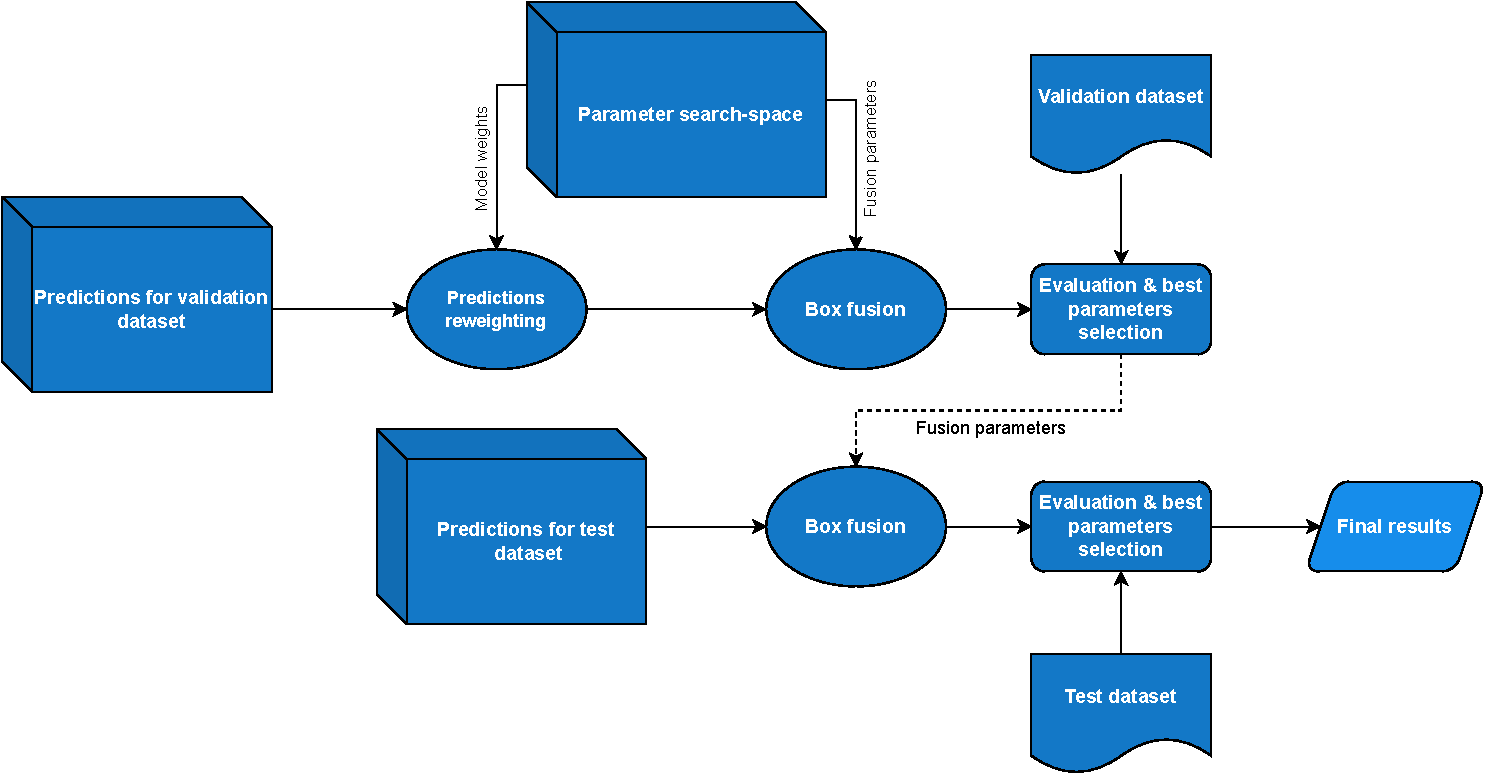
\includegraphics[width=\linewidth]{images/ensemble_search_diag.drawio.pdf}
    \caption{Schema of the search of hyper-parametrs and weights for ensembling}
    \label{fig:diag:ense_search}
\end{figure}

\subsubsection{Grid-search}
\label{sec:ens_grid_search}
Grid search over hyper-parameters was performed in the following manner: Parameter search space was defined, it can be seen in table \ref{tab:ensembling_search_space}. We evaluated $AP@.5$ on every image of the validation dataset and averaged those values. The best hyper-parameters were selected, and we used them for evaluation on the test dataset. The whole workflow is shown in figure \ref{fig:diag:ense_search}.
\begin{table}
    \centering
    \begin{tabular}{|c|c|c|c|}
        \hline
        Parameter    & minimal value & maximal value & step \\ \hline
        Model weight & 0.12          & 1             & 0.22 \\ \hline
        IOU $T$      & 0.3           & 0.9           & 0.05 \\ \hline
        Sigma        & 0.3           & 1             & 0.1  \\ \hline
    \end{tabular}
    \caption{Hyper parameter search-space for area-aware model ensembling}
    \label{tab:ensembling_search_space}
\end{table}

\subsection{Area-aware ensembling}
\label{sec:methods_area_aware_ens}
We propose a change to the weighting function in ensembling; see equation \ref{eq:ensembling_weighting}. The new weighting function described in equation \ref{eq:ensemble_weighting_area} is aware of the area of ensembled boxes. We hypothesize that this would increase the modeling capacity of the ensemble methods.

The equation \ref{eq:ensembling_weighting} was changed to:
\begin{align}
    \mathcal{S} = \bigcup_{i=1}^{M} \frac{S_i f(B_i, \mathbf{w_i})}{ F}, \quad
    f(B_i, \mathbf{w_i}) = \begin{cases}
        w_1,\quad \text{area}(B_i) \leq 32^2        \\
        w_2,\quad 32^2 < \text{area}(B_i) \leq 96^2 \\
        w_3,\quad 96^2 < \text{area}(B_i)           \\
    \end{cases}
    \label{eq:ensemble_weighting_area}
\end{align}
We tried to perform a grid search with the equation \ref{eq:ensemble_weighting_area} used for the weighting of boxes, but the number of parameters grew exponentially, making the grid search computationally untractable. We, therefore, used the Optuna optimization library to perform this task. The search space is in table \ref{tab:ensembling_search_space_area}; please note that the search space became continuous contrary to the previous.

\begin{table}
    \centering
    \begin{tabular}{|c|c|c|}
        \hline
        Parameter                           & minimal value & maximal value \\ \hline
        Model weight (small, medium, large) & 0.01          & 1             \\ \hline
        IOU $T$                             & 0.05          & 1             \\ \hline
    \end{tabular}
    \caption{Hyper parameter search-space for model ensembling}
    \label{tab:ensembling_search_space_area}
\end{table}


\subsection{Assessing importance of different models in ensembling}
\label{sec:methods:assesing_importance}
To get an insight into what affects the performance of model ensembling, we compare the following: an Ensemble of multiple models with the same architecture and backbone, an ensemble of models with the same architecture and different backbones, and an ensemble of different architectures. All models selected for ensembling were trained on the stage five dataset, including the changes proposed in section \ref{sec:general_changes}. The results of a subset of those models are in Table \ref{tab:improved:precision}.


After selecting models, we ensembled them using the WBF method. Model weights and IOU threshold $T$ value were optimized on the validation dataset as described in section \ref{sec:ens_grid_search}. The Optuna optimization software was used to find those, where we set search-space to be in the range from 0 to 1 for all model weights as well as for the IOU threshold $T$. The optimization process was terminated after $3000$ trials.

After obtaining the ensembles, we assess the importance of each model included in the ensemble by a method based on functional analysis of variance (FANOVA) \cite{Hutter2014}. We used an already implemented solution that is part of the Optuna library \cite{Akiba2019}.
\subsubsection{The same architecture and backbone}
We used YOLOv5 architecture with a medium sized backbone, since multiple models were trained for experiments mentioned in section \ref{sec:model_inspection}. Summary of used models is available in table \ref{tab:ensemble_models_involved}.

\subsection{The same architecture different backbones}
We used YOLOv5 architecture again but included two models with a small backbone, three with a medium-sized backbone, and three with the large backbone. When picking those, we tried to match the performance of selected models with those selected before. This was done to ensure the maximal comparability of those two ensembles.

\subsection{Different architecture}
Here we used the best model we had at our disposal. The ensemble consisted of the following models: Two YOLOv5-large, two YOLOv5-medium, YOLOv5-small, EfficientDet-D1, EfficientDet-D3, RetinaNet-swint, and Faster-RCNN-Resnet50. Even though we picked the best available models, the difference in $AP@.5$ against YOLOv5-all was $2\$$, as can be seen in table \ref{tab:ensemble_models_involved}, where we denoted a group of models with different architectures as All.

\begin{table}[h]
    \centering
    \begin{tabular}{|c|c|c|c|c|c|}
        \hline
        Experiment & num.models & mean  & std   & min   & max   \\ \hline
        YOLOv5-m   & 8          & 0.696 & 0.014 & 0.668 & 0.719 \\ \hline
        YOLOv5-all & 8          & 0.693 & 0.017 & 0.659 & 0.719 \\ \hline
        All        & 10         & 0.707 & 0.014 & 0.676 & 0.725 \\ \hline
    \end{tabular}
    \caption{Comparison of models envolved in ensembling by statics of their $AP@.5$ metrics}
    \label{tab:ensemble_models_involved}
\end{table}

\section{Dental-restorations segmentation segmentation}
\label{sec:methods:dental_restorations}
In this section, we propose a non-deep learning method for the segmentation of dental caries; we tune hyper-parameters of this approach to achieve the best possible performance of this approach. After that, we switched our approach and trained a deep learning model called U-Net.
\subsection{Non-deep learning approach}
\label{sec:methods:seg_nondl}
We decided to test the approach proposed by Abdalla-Aslan, and Yeshua \cite{AbdallaAslan2020, Yeshua2019} as described in section \ref{sec:related_works:dental_restorations}. This means that we defined a pipeline of image processing operations, where we:
\begin{itemize}
    \item Thresholded the image: We tried Otsu's thresholding method and Gaussian blur with kernel size $K_b$ applied prior to that. Furthermore, Gaussian and mean adaptive thresholding methods were tried, where we tested different kernel sizes $K_t$ and threshold values $T$.
    \item Removed predicted pixels at the border of the X-ray image: Bitewing X-ray images usually do not have a rectangular shape, as can be seen in \ref{fig:bitewing_sample}. Bitewing radiographs are therefore padded with black color to obtain the rectangular shape. This leads to a high contrast at the border of the radiograph, which gets detected by adaptive thresholding methods. We, therefore, detect this padding and morphologically dilate it by the square kernel of size $K_d \times K_d$. Border pixels obtained by dilation are removed from the thresholded image.
    \item Morphological opening: We apply morphological opening to filter out falsely detected regions; we use a square-shaped kernel with size $K_o$.
\end{itemize}

The pipeline defined above has four hyper-parameters to be tuned and three thresholding methods. We therefore define a grid-shaped search space as can be seen in table \ref{tab:hyper_param_segmentation}. Note that when we searched for the value of $K_t$ we did not search for $K_b$ and vice versa.
The dataset was split into two equally-sized parts, called tune and test. We evaluated the IOU metric on each image of the tune part of the dataset and averaged it for each set of hyper-parameters. We selected the best hyper-parameters based on the average IOU value and used those to evaluate on the test part of the dataset.

\begin{table}
    \begin{tabular}{|c|c|c|c|}
        \hline
        Hyper-parameter & minimal value & maximal value & step \\ \hline
        $K_t$           & 33            & 83            & 10   \\ \hline
        $K_b$           & 1             & 26            & 5    \\ \hline
        $T$             & 1             & 15            & 2    \\ \hline
        $K_d$           & 41            & 81            & 20   \\ \hline
        $K_o$           & 1             & 36            & 5    \\ \hline
    \end{tabular}
    \caption{Hyper-parameter search space for restorations segmentation pipeline}
    \label{tab:hyper_param_segmentation}
\end{table}

\subsection{Deep-learning approach}
\label{sec:methods:seg_unet}
\subsubsection{Model training}
The dataset was split into training, validation, and test parts with a 70:15:15 ratio. For the dataset's training part we used augmentations described in section \ref{sec:image_augmentations}. Resizing of images was removed from the augmentation pipeline, and we, therefore, worked with full-sized radiographs. Images in the validation and test part of the dataset were only normalized.
We used the U-Net architecture model as proposed by author \cite{Ronneberger2015}, only changing the depth to 5 downscaling layers. As a loss function, we used Soft-dice loss. The learning rate value of $10^{-2}$ was used together with reduce on plateau learning rate scheduler. The model was trained for 50 epochs by the Adam optimizer, and at the end of the training, we selected the best model according to IOU on the validation dataset and evaluated its performance on the test dataset.

\subsubsection{Post-processing}
\label{sec:segmentation_post_processing}
On the best-performing model, we used post-processing methods inspired by the non-deep learning approach. The image was first morphological opened by a square kernel with a size of $K_O$ and then closed by a kernel size of $K_C$.

Since there were two hyper-parameters involved, we performed a grid-search, searching for the kernel of size from 1 to 41 with the step size of 4. Firstly we saved predictions for all images in the validation dataset. This ensured that we did not have to pass the image thru the U-Net model for each parameter. Post-processing with all defined kernel values was applied. The best-performing hyper-parameters were selected, and post-processed predictions were evaluated on the test dataset.

\subsection{Model training improvements}
We tried the following changes to the model training pipeline:
\begin{itemize}
    \item AdamW optimizer was used insted of Adam
    \item Cosine annealing learning rate scheduler was used. The half-period of cosine was set to 40 epochs and the minimal learning rate was set to $10^{-7}$.
    \item Binary cross-entropy loss was tested instead of Soft dice loss as well as a combination of Soft dice loss with BCE.
    \item We removed the maximal amount of epochs and instead used the IOU value on the validation set as a stopping criterion. Whenever no improvement of IOU was observed for ten epochs, the training was stopped.
\end{itemize}

After the training, we performed the same post-processing. We found the best hyper-parameters by the Optuna optimization library. The search space ranged from $1$ to $41$ for both kernels.


